% -*- TeX-command-extra-options: "-shell-escape"; -*-
\documentclass[convert={density=1200,size=1080x800,outext=.png}, tikz]{standalone}
\usetikzlibrary{calc}
\usepackage{pgfplots}
\pgfplotsset{compat=1.18}
\begin{document}
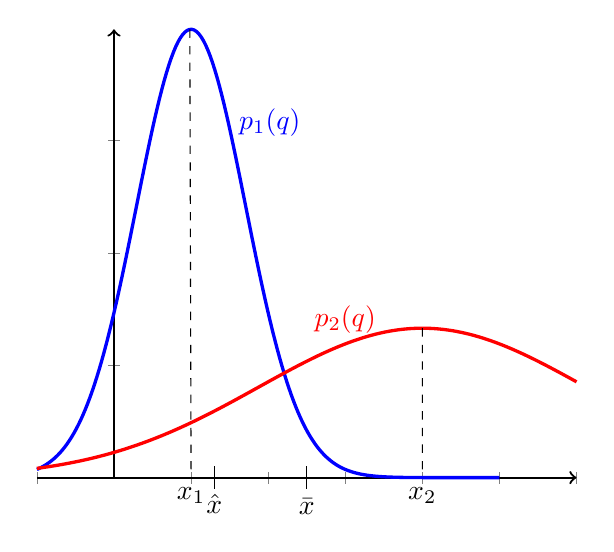
\begin{tikzpicture}[
    small dot/.style={fill=black,circle,scale=0.3},
  ]

  \begin{axis}[
    clip=false,
    xticklabels={},
    yticklabels={},
    axis lines=center, % Draw the axes through the center
    axis line style={->, thick}, % Arrow style for axes
    xmin=-1,xmax=6
    ]
    % density of Normal distribution:
    \addplot [
        blue,
        domain=-1:5.0,
        samples=201,
        very thick
    ]
        {exp(-(x-1)^2 / (1^2)) / (1 * sqrt(2*pi))} coordinate[pos=2/6] (blue-peak) node[pos=2.5/6, anchor=west] {$p_{1}(q)$};
    \addplot [
        red,
        domain=-1:6,
        samples=201,
        very thick
    ]
        {exp(-(x-4)^2 / (3^2)) / (3 * sqrt(2*pi))} coordinate[pos=5/7] (red-peak) node[pos=4/7, anchor=south] {$p_{2}(q)$};

    \coordinate (ll) at (axis description cs:0,0.0);
    \coordinate (one) at (axis cs:1,0);
    \coordinate (four) at (axis cs:4,0);
    \draw[dashed] (blue-peak) to (ll -| one) node[anchor=north] {$x_{1}$};
    \draw[dashed] (red-peak) to (ll -| four) node[anchor=north] {$x_{2}$};

    \draw (axis cs:2.5,0.01) to (axis cs:2.5,-0.01) node[anchor=north] {$\bar{x}$};
    % julia> (1/1*1+1/9*4)/(1/1+1/9)
    % 1.2999999999999998
    \draw (axis cs:1.3,0.01) to (axis cs:1.3,-0.01) node[anchor=north, inner sep=1.8] {$\hat{x}$};
  \end{axis}

\end{tikzpicture}
\end{document}
